%The interaction design of the clients, what principles has been used. Directed towards developers. Start with subsection here. Android and iOS need to start with subsubsection.

This chapter goes into detail on how the graphical and interactive parts of the clients are designed. It starts with a general view of the interaction design and then divides into chapters based on the different clients.

\section{General view}
Since the Genomizer application is first and foremost about handling important 
data, it is crucial to allow the user to be in control but still to protect 
and preserve the data that is already in the system from non-authorized users.
That is why Genomizer uses a log in screen to reassure that only authorized 
personnel can access the server data.

The workflow of Genomizer is intended to be as natural as possible for 
the users and to be easily integrated into their daily work routine.
Furthermore, simplicity is favored, the clean and consistent design 
facilitating the tasks without adding the distraction of any 
unneccessary features.

%\footnote{\url{http://en.wikibooks.org/wiki/GUI_Design_Principles}}

\section{Desktop client}
Screen clients use a tab based navigation between views, these tabs are shown at the top of the user interface. The common views in the current system are search, upload and process.

Search results are displayed in a table, experiments can be expanded to reveal the files contained in the experiment. The files in an experiment are grouped by types where each type consists of a row in the table that may be expanded to reveal the files of that type.

The upload view consists of experiment groups. Each experiment group contains a set of input fields for annotation and a list of files added to this experiment. The user may create new experiments in this view or add files to an existing experiment, multiple files may be added to multiple experiments simultaneously.

The base for the process view contains a set of input fields for the parameters that are to be used when processing a file.

\FloatBarrier
\subsection{\term{Windows}/\term{OS X}/\term{Linux} application}
The first thing a user will see when starting the desktop client is the login window (see \refer{fig:des_login_window}). The window prompts the user for user name, password, and a server IP to connect to. If the correct credentials are entered, the user will be logged in and taken to the next screen. If the user enters an invalid password, user name, or server, an appropriate error message will be displayed as seen in \refer{fig:des_login_failed}. This feedback informs that user the login was unsuccessful.
\begin{figure}[h]
	\addScaledImage{0.9}{des_login_window.png}
	\caption{The login window.}
	\label{fig:des_login_window}
\end{figure}
\begin{figure}[h!]
	\addScaledImage{0.9}{des_login_failed.png}
	\caption{The login window with an error message after a failed login.}
	\label{fig:des_login_failed}
\end{figure}
\\\\
After the user has been successfully logged in, the main window will appear (see \refer{fig:des_main_window}). The main window  is built with tabs to simplify work by letting the user easily switch between different views for different work tasks. Each tab is described by appropriate name and contains related functionality. The main window also has a log out button. This button is of little importance, and is therefore located in the upper right corner.
\\\\
At the bottom of the main window a status panel is located. The status panel gives feedback from different tasks executed by the user. When a task is executed successfully, the color of the status bar will turn green, and display a message. In case of an unsuccessful execution, the status bar will turn red, to indicate that something went wrong.
\begin{figure}[h]
	\addScaledImage{0.5}{des_main_window.png}
	\caption{The Genomizer desktop client's main window. The window have tabs for different views (1), a log out button (2), and a status panel for feedback (3).}
	\label{fig:des_main_window}
\end{figure}

From the search view (see \refer{fig:des_search_tab_interaction}) the user can build search queries and look up existing experiments. The search view has been designed to have a similar layout and interaction as the advanced search tool on the site \\ \href{http://www.ncbi.nlm.nih.gov/pubmed/advanced}{http://www.ncbi.nlm.nih.gov/pubmed/advanced}
. The researchers are familiar with this site, so they can recognize interaction elements from it when using the search function of the desktop client.
\\\\
To search for experiments the user can click the magnifying glass. This icon is well-known and often associated with searching. The icon is located next to the search field, so that the user can easily understand that the search field and the icon are connected. The user can also press the enter key to perform a search, without letting go of the keyboard, making the interaction faster. Next to the magnifying glass is a button for emptying the search field. The button has an icon depicting a trash can -- a well-known metaphor for removing or emptying things.

\begin{figure}[h!]
	\addScaledImage{0.7}{des_search_tab_interaction.png}
	\caption{The search view of the Genomizer desktop client with the icons for search and emptying the search field highlighted.}
	\label{fig:des_search_tab_interaction}
\end{figure}

From the upload view (see \refer{fig:des_upload_view}) the user can create new experiments and upload files to them. When creating a new experiment the user is forced to fill in some fields. These fields have been given a bold-texted label, to indicate that they are of more importance than the others. A text below the fields also states that bold fields are forced. Non-forced fields are labeled with non-bold text.

To inform the user that information is missing, constraints has been put on the buttons for creating the experiment. If any forced field has not been filled in, or no files have been added for upload, these buttons will be grayed-out and cannot be clicked.

For each file added to the experiment there is a progress bar. This bar gives the user feedback on upload process. Each file also has  its size displayed after its name. This gives the user an idea of how time consuming the upload will be.

\begin{figure}[h!]
	\addScaledImage{0.6}{des_upload_view.png}
	\caption{The upload view of the Genomizer desktop client. An empty forced field (1), as stated by the bold-texted label (2), makes the upload buttons (3) grayed-out. The upload progression bar (4) and the size of the file (5) gives the user an idea of how time consuming the uploading process will be.}
	\label{fig:des_upload_view}
\end{figure}

The workspace tab lets the user easily manage files and experiments. Files and experiments in the work space are listed the same way as search results in the search view, making the design consistent throughout the system. The workspace view has easy access to the download and process functions.

The administration view (see \refer{fig:des_admin_view}) is divided into two seperate views, one for managing annotations and the other one for managing genome releases. The division of the views makes the interface less cluttered and less confusing, and also increases the cohesion of the views. The user can easily switch between the views by clicking the the tabs on the left-hand side.

\begin{figure}[h]
	\addScaledImage{0.9}{des_admin_view.png}
	\caption{The administration view showing part of the view for managing annotation. The highlighted tabs to the left let's the user switch between views.}
	\label{fig:des_admin_view}
\end{figure}

To improve the feedback when errors occur, an error dialog (see \refer{fig:des_error_dialog}) will be shown. The dialog explains what went wrong and why the error occurred. The user can find additional information about the error by clicking a button labled 'More info'. This information can be useful for system administrators, developers or support, but not for regular users (which is why it is initially hidden).

\begin{figure}[h!]
	\addScaledImage{0.6}{des_error_dialog.png}
	\caption{An error dialog that explains that the user have entered invalid characters for an experiment name.}
	\label{fig:des_error_dialog}
\end{figure}

\FloatBarrier



\FloatBarrier
\section{Web application}
% WHAT?
% WHY?
% User story compatibility 

Generally, the design of the user interface for the web application is an integration of the principles previously described with core design elements of web and the twitter bootstrap element library. 

\subsubsection{Layout and Structure}
The structure of the application is in most cases shallow, the navigational depth is usually two steps but sub views with modal views may result in a depth of 3. There are three types of views which are hierarchical in some way, main views contain sub views and modal views, sub views may contain modal views.

\begin{itemize}
    \item \textbf{Navigation bar:}
A navigation bar is a menu that contains an overview of the functionality in the form of, in this case, tabs that leads the user to other views and that is always visible for the user to allow easy navigation. The navigation bar for the application can be seen in \autoref{adm_web_annotationView1}. Since the most important parts of the application is to be able to upload, process and convert files, these are each a natural part of the navigation bar (although conversion is not yet implemented and therefore not shown in the figure).

\begin{figure}
 \centering
 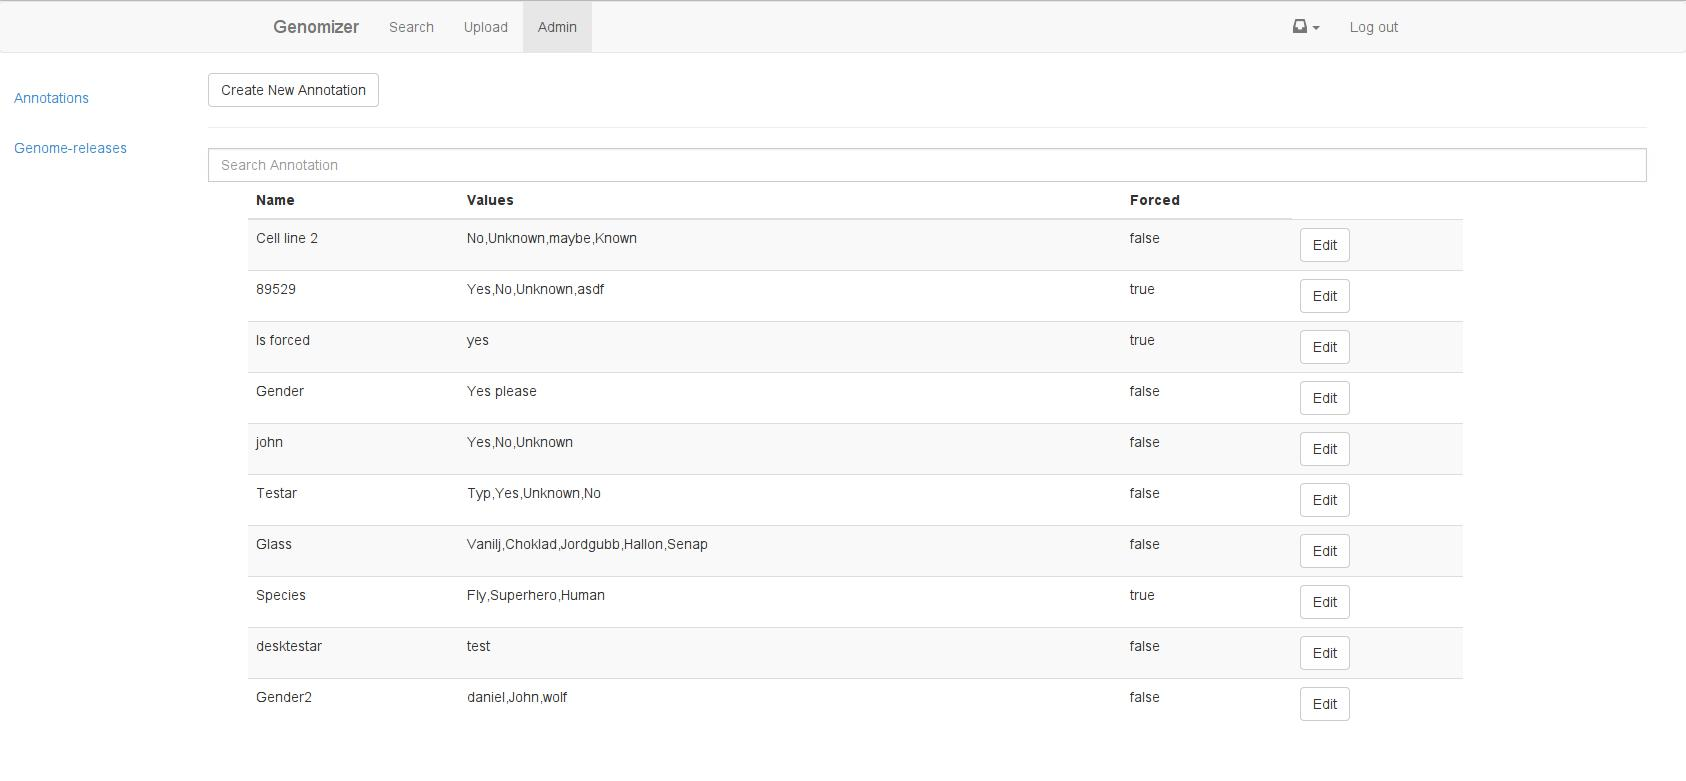
\includegraphics[trim=40 260 45 50, clip, width=0.8\textwidth]{web_SysadminAnnotationView.jpg}
 \caption{The web client navigation bar.}
 \label{adm_web_annotationView1}
\end{figure}

	\item \textbf{Main views:}
A main view covers the entire page except for the navigation bar. The structure among main views is shallow and the user may freely navigate between all main views using the navigation bar. Typically a main view contains a toolbar and a set of panels. \autoref{adm_web_annotationView2} shows the administration main view.

\begin{figure}
 \centering
 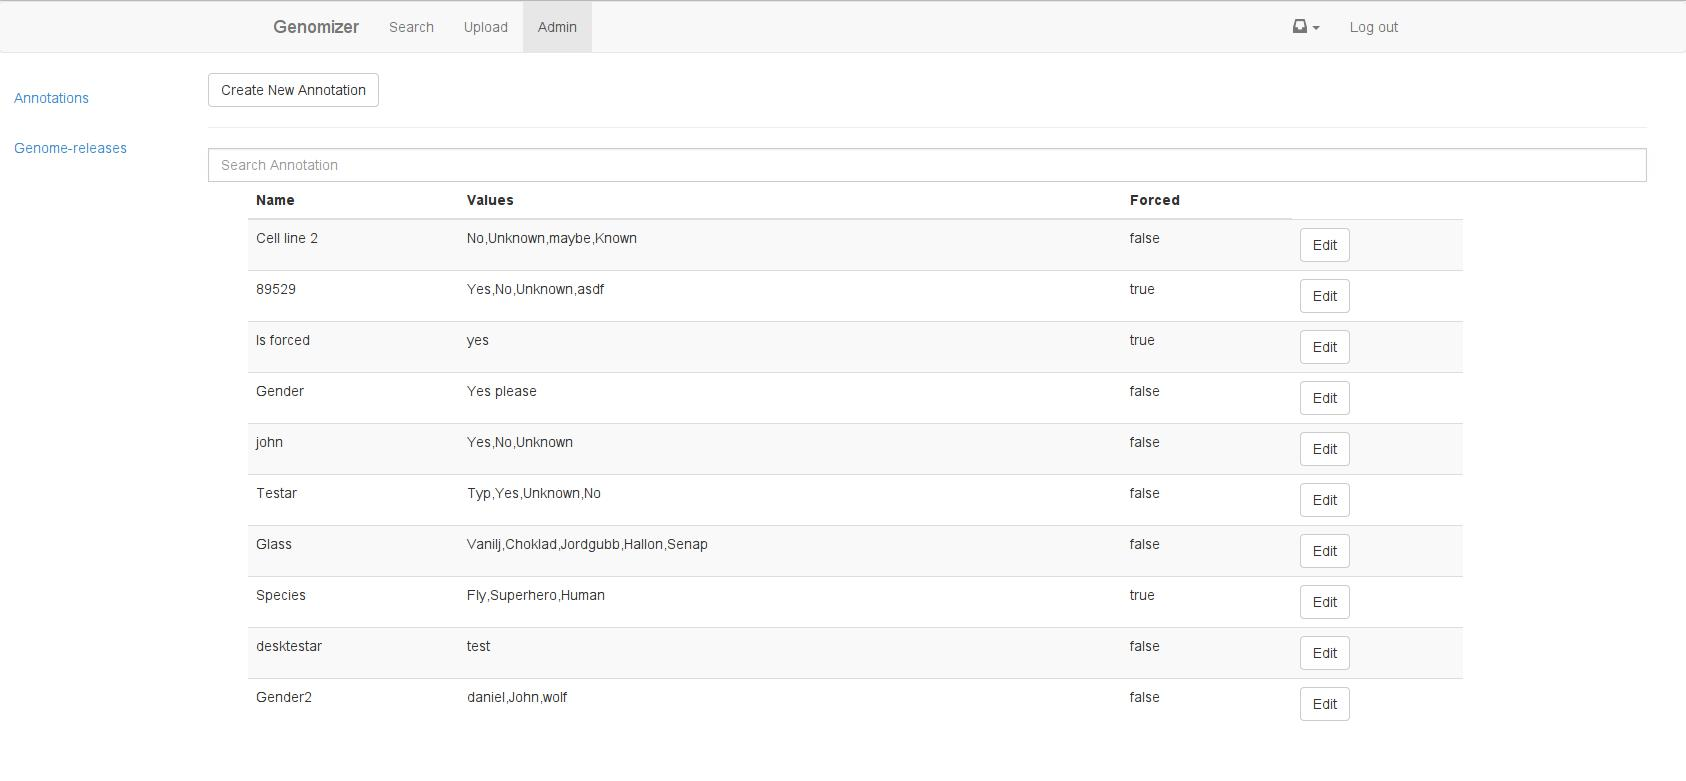
\includegraphics[width=\textwidth]{web_SysadminAnnotationView.jpg}
 \caption{The web client administrator main view.}
 \label{adm_web_annotationView2}
\end{figure}

	\item \textbf{Sub views:}
A sub view is a part of a main view. In the case of the administrator view seen in \autoref{adm_web_annotationView2}, the main view has a vertical navigation bar on the left side used to navigate between sub views, sub views may not be directly navigated outside of its main view. The user may navigate to other main views from a sub view. Except for the sub navigation bar the sub view covers the entire main view, replacing its content, as does the annotation view in this case.

	\item \textbf{Modal views:}
Modal views are opened on top of the current main view and are used for specialized operations. Modal views can be navigated to using buttons inside main views and sub views. Usually the user will be taken back to the previous view when the modal is closed but navigation in a sequence of modal views could be implemented in the future. An example
of a modal view is the login view seen in \autoref{fig:web_search_login1}.

\begin{figure}
\centering
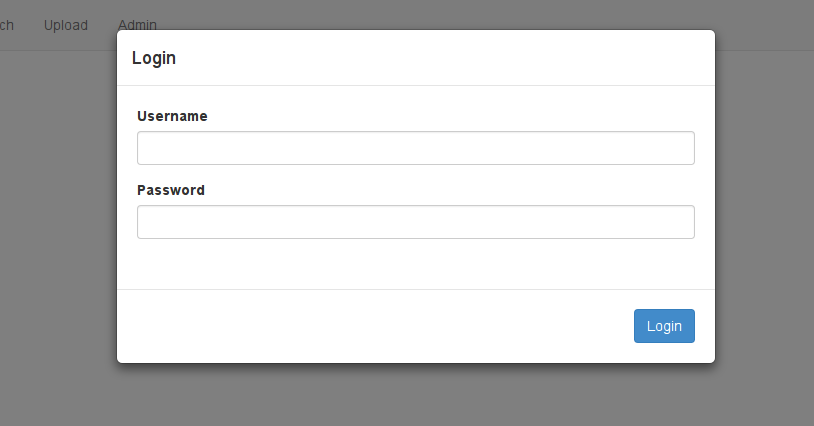
\includegraphics[width=0.8\textwidth]{web/manual/web_login.png}
\caption{The login modal.}
\label{fig:web_search_login1}
\end{figure}

    \item \textbf{Panels:}
Content that belongs together is grouped using so bootstrap panels. Main views and sub views should contain one or more panels.
    
    \item \textbf{Toolbars:}
In main views and sub views we use a toolbars where operation controls available to the user are presented, for example, add and search experiment functionality in the upload view.
    
    \item \textbf{Popovers:}
Elements that belong to a view but have no need to be visible at all times are shown in bootstrap popovers. Popovers that do not belong to a specific view may be placed in the navigation bar, that is, the main menu.
\end{itemize}

\subsubsection{Colors}
Grayscale colors are mostly used, black or dark gray is used for text, icons and borders while white or light gray is used for backgrounds. Colors of different hues are used to distinguish elements from each other and to highlight important elements. Colors with high saturation are reserved for smaller elements while colors with lower saturation can be used regardless of element size. Light gray of varying brightness may also be used to highlight or distinguish elements.

\subsubsection{Icons}
Buttons that perform actions should always contain an icon as well as text so that the experienced user may more quickly desired actions by identifying buttons at a glance instead of having to read the button text. 

\subsubsection{Batching}
For operations performed on objects that there are multiples of e.g. experiments or files, let the user perform these operations on multiple objects at the same time in cases where it makes sense using checkboxes.

\subsubsection{Processing}
The interaction flow of the processing is adapted from the actual processing 
steps in order to help the researchers by increasing usability through providing
a well-known but more optimized approach.

After having chosen an experiment for processing and entered the processing 
view, the user can choose the processing steps wanted and enter the correct
files and parameters for each processing step as shown in .


\FloatBarrier
\section{Android}
%\subsection{Interaction Design}

%The design of the Android application is based on the design proposal suggested by the design team and our aim has been to recreate that look and feel. We did, however, find it necessary to take into consideration some of the Android specific design paradigms which distinguish Android applications from other smart phone platforms. For instance, the design put forth by the design group did not include a so called action bar   to the upper part of the user interface which are used for navigation. However, since these are fundamental to the structure of any Android application, we were inclined to include this feature as a substitute for the slide-in menu described in the original design.

%In the following sub-sections, we will attempt to explain our design desisions.

The \appName\ \textit{Android} application was designed to allow for a quick search of the database while on the move. It also makes it possible to start processes in advance so that the data is ready when further work and analysis is to be done. The application will also provide a way to continuously view the status of active processes on the server. 

The application was designed in close collaboration with the \term{iOS} application in order to provide a consistent experience on both plattforms.  We did, however, find it necessary to take into consideration some of the \textit{Android} specific design paradigms which distinguish \textit{Android} applications from other smart phone platforms. In this section the layout and design decisions will be described.


\subsection{Login view}
There are two textfields available for the user to type username and password and a button to click when user is ready to log in.
This is a popular layout for many login screens and thus a design many users are familiar with.


\begin{figure}[ht]
\addScaledImage{0.2}{figures/and_login.png}
\caption{\footnotesize Login view}
\label{fig:and_login}
\end{figure}
\FloatBarrier

\subsection{Search view}
The design illustrated in \refer{fig:and_search} show the search view, 
which is also the view the user is presented with upon successful login.
The search annotations are displayed in a list and it is easy to learn how to search.
Scroll bars are used for multiple options and textfields are used for free text. 
At the bottom of the view there is a button to press in order to start the search.

\begin{figure}[ht]
\addScaledImage{0.2}{figures/and_search_regular.png} 
\caption{\footnotesize Search view}
\label{fig:and_search}
\end{figure}
\FloatBarrier

\subsection{Search result view}
The design illustrated in \refer{fig:and_result} show the search result view. 
The result is shown in a list, sorted by experiments. The list displaying search results is large to facilitate usage for user and to take advantage of the screen space. 
It is easy to learn how to navigate the list. 
Scrolling is available if the list is long and if the user clicks on an experiment they are redirected to the experiment view displaying more information about that experiment.

\begin{figure}[ht]
\addScaledImage{0.2}{figures/and_search_result.png} 
\caption{\footnotesize Search result view}
\label{fig:and_result}
\end{figure}
\FloatBarrier

\subsection{Experiment view}
The design illustrated in \refer{fig:and_experiment} shows more information about a specific experiment. 
All files associated with the experiment is displayed here and sorted by type (raw, profile and region).
The button \click{Go to process} at the bottom takes the user to the process view, where the user can process all raw files associated with the experiment.
If no raw files should exist, the button will be disabled.

\begin{figure}[ht]
\addScaledImage{0.2}{figures/and_result_experiment.png} 
\caption{\footnotesize Experiment view}
\label{fig:and_experiment}
\end{figure}
\FloatBarrier

\subsection{Search settings view}
The design illustrated in \refer{fig:and_search_settings} is showing the view for search settings. 
This is a way for the user to select annotations to be displayed in the search result view.
The user can select annotations by checking the checkbox next to the annotation name.
The user can also select on how to sort the experiments.
This functionality gives the users the possibility to design the search result view the way they want to have it, which often is appreciated. 

\begin{figure}[ht]
\addScaledImage{0.2}{figures/and_search_select_visible_annotations.png} 
\caption{\footnotesize Search settings view}
\label{fig:and_search_settings}
\end{figure}
\FloatBarrier

\subsection{Process view}
The design illustrated in \refer{fig:and_processing_view} is showing the view for processing. 
This enables the user to start a process from raw to profile. The only selectable input files are the ones that exist in the experiment.
The \click{Parameters} button enables the user to change the \verb!Bowtie! flags.
The plus icon in the action bar adds a new entry, and the cross removes the associated entry.

\begin{figure}[ht]
\addScaledImage{0.2}{figures/and_processing_view.png} 
\caption{\footnotesize Processing view}
\label{fig:and_processing_view}
\end{figure}
\FloatBarrier

\subsection{Active processes view}
The design illustrated in \refer{fig:and_active_processes_view} is showing the view for active processes on the server. 
The user is automatically navigated here when the \click{Process} button in the process view is clicked.
The user can here choose to remove any process on the server.

\begin{figure}[ht]
\addScaledImage{0.2}{figures/and_process_status.png} 
\caption{\footnotesize Active processes view}
\label{fig:and_active_processes_view}
\end{figure}
\FloatBarrier


\FloatBarrier
\section{iOS}
Focus has been on making a nice looking application with an intuitive workflow and to follow the iOS design principles. Some of the design decisions are motivated in the text below.

\subsection{Navigation bar}
A navigation bar is used to make access to different main functionalities available at all times. Big and clear icons are used to show the user which view they all represent. It is also possible to simply swipe between the different views to increase the speed of which the advanced user can use the system.

\subsection{Login Screen}
The login screen has two responsibilities; to make a nice first impression and to make it easy for the user to login. The design is kept simple and clean to avoid distractions.

\subsection{Search View}
The search view is designed to be usable for both advanced and new users. A list with available annotations is displayed to make it easy to do basic searches fast. Some annotations can only be selected with a picker view, while others are edited by typing free text. The reason for the occurance of the picker views is to simplify searches and help the user to make correct search requests. For example, the sex of an individual can only be male, female or unknown. Other values for the sex annotation would be nonsence! The search button disappears when no annotation is selected to decrease the chance of user sending empty searches and to increase the understanding of the switches. 

\begin{figure}[ht]
\addTwoImages	{ios_search1.PNG}{a}
		{ios_search2.PNG}{b}
\caption{The search screen.}
\label{fig:ios_search2}
\end{figure}
\FloatBarrier

Each annotation has a corresponding switch button as seen in \refer{fig:ios_search2}a-b. The button determines if the annotation should be included in the search request. This make it easy to make small changes to the search, while not clearing the annotation values.

The advanced user can customize the search query sent to the server. This gives the user the possibility make more complex search queries and possibly make use of already accuried PubMed-search skills.

\subsection{Search Result View}
The main purpose of the search result view is to give an overview of the search results. The challenge with this view was to summarize large amount of information in a small area. The small screen of the iPhone made it impossible to have columns for each annotation. Instead a decision was made to group the files by experiment as seen in \refer{fig:ios_searchResult2}. The table with the experiments will only expand vertically, both when the number of shown annotations and the number of experiments grows. Thus, the user never has to scroll sideways which would be awkward.

\begin{figure}[ht]
\addScaledImage{0.30}{ios_result3.PNG}
\caption{The search result view.}
\label{fig:ios_searchResult2}
\end{figure}
\FloatBarrier

The user can choose which annotations to display in the result view. This gives the user the possibility to only show the annotations which are interesting at the moment. 

The files view (see \refer{fig:ios_files2}a), which is shown when the user selects an experiment, only contains the filename of the files in the specific experiment. The annotations is not shown in this view to avoid information overload and to give the user a good overview of the files. The purpose of the plus-symbol next to each file is to add as many files as the user wish to use when selecting processes. More information can be seen when the circled 'i' to the left of the filename is tapped, an example of this can be seen in \refer{fig:ios_files2}b. 

\begin{figure}[ht]
\addTwoImages	{ios_process_files.jpg}{a}
		{ios_files2.PNG}{b}
\caption{The file view.}
\label{fig:ios_files2}
\end{figure}
\FloatBarrier


% The functionality of the Convert files button can be reached from other views, but was added to this view as well to improve the workflow. Instead of first selecting the files, then going to the Selected files view and initiate the convertion from there, the user can quickly convert files directly from the search results.

%\subsubsection{Selected Files}
%The selected files view can be seen in \refer{fig:ios_selectedFiles2}a. The files are grouped into four categories: raw, profile, region and other. This is done by showing each type of files in its own tab located at the top of the screen. The reason for this is to avoid the possibility to select files of different types since the tasks to perform are file type specific. It also gives a better overview of the files when only one type is shown instead of showing all files at the same time. The files are also grouped into respective experiment they belong to. This is done to avoid confusion of what file belong to which experiment with similar filenames etc. Additionally, the top navigation bar menu is following the iOS design guidelines. 
%
%When at least one file is selected with the switch next to it (see \refer{fig:ios_selectedFiles2}b) a button will appear at the bottom of the screen letting the user choose a task to perform with the file by leading to the select task menu, as seen in \refer{fig:ios_convertParameters}a.
%
%\begin{figure}[ht]
%\addTwoImages	{ios_selected1.PNG}{a}
%		{ios_selected2.PNG}{b}
%\caption{The selected files view.}
%\label{fig:ios_selectedFiles2}
%\end{figure}
%\FloatBarrier


\subsubsection{Create processes}
The view to create a process is focused on the user's current workflow. The user wants to use the selected files from the files view as input and then select a specific process on those files, which creates output-files to be used as input-files in another process. This creates a sequence of processes which the server will execute one process at a time. Moreover each input-file for a process will be executed parallel with eachother. The input-files and the output-files are separated by the process which will be executed on the input-files. To make it easy to understand what will be executed on each step of the sequence the separator between input-files and output-files is the name of the process and an arrow from the input-files to output-files. The color of a output-file will have the same color as its corresponding input-file to track a file's conversion-process, from start to finish, see \refer{fig:ios_creating_process}a-c. 



\begin{figure}[ht]
\addThreeImages {ios_empty_make_process.jpg}{a}
	{ios_one_process.jpg}{b}
	{ios_many_process.jpg}{c}
\caption{Creating a process}
\label{fig:ios_creating_process}
\end{figure}
\FloatBarrier

\subsubsection{Processes}

As visible in \refer{fig:ios_processingStatus}, we chose to build the processing status view with a simple tableview, to make it dynamic and easy. We also think this gives the user the best possible overview of current processes. The status is color coded to make it as easy as possible for the user to see which processes are in which state.
\begin{figure}[h]
\addScaledImage{0.30}{ios_processes1.PNG}
\caption{The process status view.}
\label{fig:ios_processingStatus}
\end{figure}
\FloatBarrier

\subsubsection{Alerts}
Alerts are simple banners animating down from the top to give the user a headsup of what is going wrong and what is going the way it is expected. The user can tap the banner to dismiss it or if nothing is done it will animate away in 2 seconds. The banners were introduced to not stop the user with prompts which the user has to react with to be able to further use the system. A red banner, as seen in \refer{fig:ios_alerts}, indicates an error and a white with a green icon, indicates something went as expected. The colors are used to allow the user to just notice which color pops down and give them somewhat of an understanding of what is going on. without having to read the text every time.
\begin{figure}[ht]
\addScaledImage{0.30}{ios_alert1.PNG}
\caption{Examples of alert}
\label{fig:ios_alerts}
\end{figure}
\FloatBarrier



